%10.9.03

\chapter{Einleitung}
Die Kenntnis der Perkolationsschwelle ist f\"ur die Vorhersage der Eigenschaften von Strukturen, die aus zuf\"allig angeordneten Objekten bestehen, sehr wichtig. Zwischen der mittleren Euler-Charakteristik solcher Strukturen und ihrer Perkolationsschwelle besteht ein enger Zusammenhang, und die mittlere Euler-Charakteristik k\"onnte daher zur Vorhersage von Perkolationsschwellen dienen. Dieser Zusammenhang wird in der vorliegenden Arbeit untersucht.
\\Zu Beginn dieses Kapitels werden Perkolationsprozesse an einigen Beispielen erl\"autert und Aspekte der Perkolationstheorie, die im weiteren Verlauf ben\"otigt werden, dargelegt. Anschlie"send wird der Befund, dass die Nullstelle der mittleren Euler-Charakteristik bei einigen Perkolationsproblemen in der N\"ahe der Perkolationsschwelle liegt, vorgestellt. Die Euler-Charakteristik wird im zweiten Kapitel ausf\"uhrlicher behandelt.
\section{Perkolation}
Um an einem Beispiel darzulegen, was man unter Perkolation versteht, betrachten wir ein leitendes Netzwerk, bestehend aus Knoten (Umspannwerke) und Verbindungen (Hochspannungsleitungen) \cite{Zallen:83}. Das Netzwerk k\"onnte zur Elektrizit\"atsversorgung eines Landes dienen. Der Einfachheit halber seien die Knoten auf einem Quadratgitter angeordnet, und jeder Knoten sei mit seinen vier Nachbarn verbunden. Eine Gruppe von Saboteuren will die Stromversorgung unterbrechen und beginnt die Verbindungen (Hochspannungsleitungen) zwischen den Knoten in zuf\"alliger Reihenfolge zu zerschneiden. Im Laufe ihrer T\"atigkeit wird Strom, der durch das Netzwerk von linken Rand zum rechten Rand flie"sen kann, immer kleiner und verschwindet, wenn exakt die H\"alfe aller Verbindungen durchtrennt ist. Das teilweise zerst\"orte Netzwerk und der Strom von linken zum rechten Rand als Funktion des Bruchteils $p$ der intakten Verbindungen sind in Abbildung \ref{fig:bondsabotage} skizziert. Anstatt die Verbindungen zwischen den Knoten zu zerst\"oren, k\"onnten die Saboteure auch die Knoten selbst angreifen. In diesem Fall gen\"ugt es, etwas mehr als 40\% der Stationen zu zerst\"oren, damit kein Strom mehr flie"st. Das Ergebnis dieses Sabotageaktes und der Strom in Abh\"angigkeit des Bruchteils der intakten Knoten sind in  Abbildung \ref{fig:sitesabotage} skizziert. Bei beiden Sabotageakten nimmt der Strom mit der Zahl der Zerst\"orungen ab und es existiert ein Wert $p=p_c$, unterhalb dessen der linke und rechte Rand nicht mehr verbunden sind, und daher kein Strom mehr flie"st. Den Wert $p_c$ nennt man Perkolationsschwelle. Bei $p=p_c$ \"andern sich globale Eigenschaften des Netzwerkes durch eine infinitesimale Variation von $p$, denn f\"ur $p>p_c$ existiert ein zusammenh\"angendes Netzwerk, das linken und rechten Rand verbindet, w\"ahrend es f\"ur $p<p_c$ nur isolierte Inseln gibt. 
\begin{figure}[tbp]
  \centering
  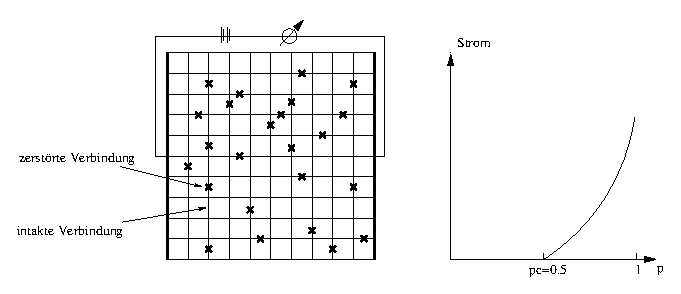
\includegraphics{./Einleitung-figs/sabobond}
  \caption{Zuf\"allige Zerst\"orung der Verbindungen eines leitenden Netzwerks: Rechts ist der Strom als Funktion des Bruchteils $p$ der intakten Verbindungen skizziert. Wenn weniger als 50\% der Verbindungen intakt sind, flie"st kein Strom mehr.}
  \label{fig:bondsabotage}
\end{figure}
\begin{figure}[bt]
  \centering
  \includegraphics{./Einleitung-figs/sabosite}
  \caption{Zuf\"allige Zerst\"orung der Knoten eines leitenden Netzwerks: Rechts ist der Strom als Funktion des Bruchteils $p$ der intakten Knoten skizziert. Wenn weniger als 59\% der Knoten intakt sind, flie"st kein Strom mehr.}
  \label{fig:sitesabotage}
\end{figure}
Ein \"ahnliches Verhalten beobachtet man in Systemen, die einen thermischen Phasen\"ubergang zeigen. Dort existiert eine kritische Temperatur $T_c$, an der sich makroskopische Eigenschaften des Systems \"andern. F\"ur $T<T_c$ existieren langreichweitige Korrelationen zwischen den Konstituenten, w\"ahrend diese Korrelationen f\"ur $T>T_c$ exponentiell abfallen. 
\\Eine scharfe Perkolationsschwelle beobachtet man aber nur in einem unendlich gro"sen System. Ist das System endlich, ist die Wahrscheinlichkeit, dass eine Verbindung zwischen gegen\"uberliegenden R\"andern existiert, f\"ur kleine $p$ nahe null, w\"ahrend sie f\"ur gro"se $p$ fast eins ist. Der \"Ubergangsbereich wird mit wachsender Systemgr\"o"se immer schmaler. Im Limes unendlicher Systemgr\"o"se wird dieser \"Ubergang scharf, und die Wahrscheinlichkeit, dass beide Seiten verbunden sind, zu einer Stufenfunktion mit Sprung bei $p_c$. 
\\Die Sabotageakte sind Beispiele f\"ur die beiden am besten untersuchten Perkolationsprozesse auf Gittern. Die Knoten entsprechen den Vertices eines Gitters; die Verbindungen zwischen den Knoten sind die Gitterkanten zwischen den Vertices. Beim ersten Sabotageakt sind alle Vertices (Knoten) vorhanden, aber nur ein Teil $p$ der Gitterkanten ist besetzt (unzerst\"ort). Dieses Modell beschreibt \textbf{bond-Perkolation}. 
Im anderen Fall ist nur ein Teil der Knoten intakt, und man nennt Vertices, die intakten Knoten entsprechen, besetzt. Benachbarte, besetzte Vertices sind durch Gitterkanten verbunden. Dieses Modell beschreibt \textbf{site-Perkolation} und der Anteil der besetzten Vertices ist die Besetzungswahrscheinlichkeit $p$. Bond- und site-Perkolation sind in ihren mathematischen Aspekten sehr \"ahnlich. In der Tat l\"asst sich jedes bond-Perkolationsproblem als site-Perkolation auf dem \"Uberdeckungsgitter (engl.: covering lattice) formulieren. Das \"Uberdeckungsgitter entsteht, indem man auf jede Gitterkante (die bonds) einen Vertex setzt, und alle Vertices verbindet, deren zugeh\"orige Kanten an einem gemeinsamen Vertex enden (siehe Abb. \ref{fig:covering_einleit}). Die physikalische Interpretation von bond- und site-Perkolation ist aber durchaus unterschiedlich.
\begin{figure}[htbp]
  \centering
  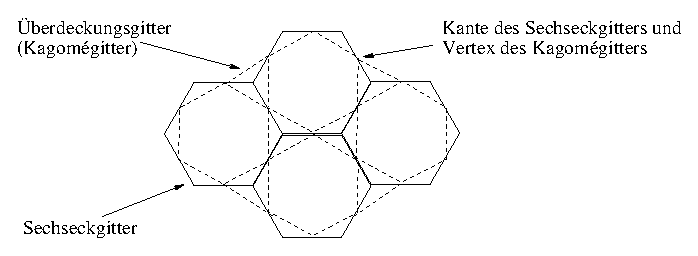
\includegraphics{./Einleitung-figs/cov}
  \caption{Das \"Uberdeckungsgitter des Sechseckgitters ist das Kagom\'egitter.}
  \label{fig:covering_einleit}
\end{figure}
\\Das bond-Perkolationsmodell wird z.B. verwendet, um den Prozess der Gelbildung zu beschreiben. Man betrachtet Monomere in einem Container und nimmt an, dass sie auf den Vertices eines Gitters angeordnet sind, und, dass sich zwischen diesen Monomeren mit einer gewissen Wahrscheinlichkeit $p$ chemische Bindungen ausbilden (siehe Abb. \ref{fig:gel}). Ist $p$ klein, existieren nur sehr wenige Bindungen, und die entstehenden Polymere sind klein. Mit $p$ wachsen die Molek\"ule. Bei $p=p_c$ entsteht erstmals ein gro"ses Makromolek\"ul, dass sich durch den ganzen Container erstreckt. Der Inhalt des Containers wird von einer Fl\"ussigkeit zu einem Gel. Das Makromolek\"ul enth\"alt aber nur einen Bruchteil der Molek\"ule und durchzieht den nach wie vor fl\"ussigen Anteil wie ein Netz. W\"achst $p$ weiter an, wird das Netz immer dichter, bis es schlie"slich bei $p=1$ alle Monomere enth\"alt.
\begin{figure}[tbp]
  \centering
  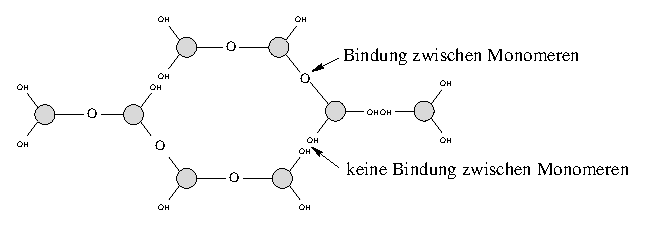
\includegraphics{./Einleitung-figs/gel}
  \caption{Monomere auf einem Sechseckgitter, zwischen denen sich chemische Bindungen ausbilden k\"onnen.}
  \label{fig:gel}
\end{figure}
\\Ein prominentes Beispiel f\"ur einen site-Perkolationsprozess ist die Modellierung von Waldbr\"anden. Die B\"aume im Wald werden durch Vertices eines zweidimensionalen Gitters dargestellt. Auf jedem Gitterplatz steht mit Wahrscheinlichkeit $p$ ein Baum, d.h. Vertices sind mit Wahrscheinlichkeit $p$ besetzt. Wenn in einen beliebigen Baum ein Blitz einschl\"agt, beginnt der Baum zu brennen. Der brennende Baum entz\"undet alle B\"aume in seiner Nachbarschaft und es entwickelt sich ein Waldbrand (siehe Abb. \ref{fig:waldbrand}). Die erwartete Anzahl $S$ der verbrannten B\"aume h\"angt von $p$ ab. Ist $p$ sehr klein, hat der Baum typischerweise keine Nachbarn und $S$ ist klein. Ist $p$ nahe eins, wird der Wald vollst\"andig verbrennen und $S$ ist unendlich. 
\begin{figure}[tbp]
  \centering
  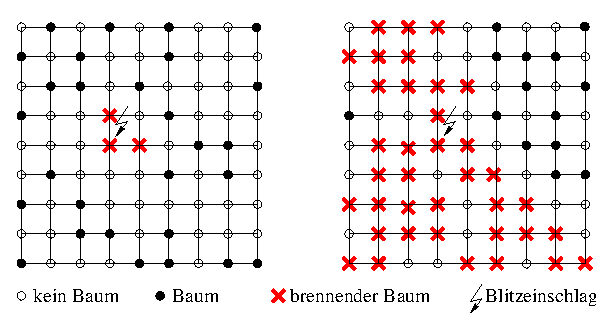
\includegraphics{./Einleitung-figs/waldbrand}
  \caption{Links: ein sp\"arlich bewachsener Wald, in dem sich der Brand nicht ausbreiten kann. Rechts: ein dicht bewachsener Wald mit gro"sr\"aumigen Brandschaden.}
  \label{fig:waldbrand}
\end{figure}
Bei $p=p_c$ \"andert sich das erwartete Schicksal des Waldes dramatisch. F\"ur $p<p_c$ existieren nur endliche zusammenh\"angende Bereiche, sog. Cluster, und der Waldbrand bleibt auf einen endlichen Cluster beschr\"ankt. Die erwartete Anzahl der verbrannten B\"aume $S$ ist die mittlere Clustergr\"o"se und f\"ur $p<p_c$ endlich. Die Wahrscheinlichkeit, dass ein Baum, der im Abstand $r$ vom Einschlagort des Blitzes steht, verbrennt, ist durch die  \textit{pair-connectedness} Funktion $\rho(r)$ gegeben. Die pair-connectedness Funktion ist die Wahrscheinlichkeit, dass zwei besetzte Vertices im Abstand $r$ zum gleichen Cluster geh\"oren. F\"ur $p<p_c$ und gro"se $r$ f\"allt $\rho$ mit $r$ exponentiell auf einer Skala $\xi(p)$ ab. F\"ur $p>p_c$ existiert ein unendlicher Cluster, und wenn der Blitz in einen Baum dieses Clusters einschl\"agt, bleibt der Waldbrand nicht auf ein endliches Gebiet beschr\"ankt. Die Wahrscheinlichkeit, dass ein Vertex zu einem unendlichen Cluster geh\"ort, wird Perkolationswahrscheinlichkeit genannt. F\"ur die Perkolationswahrscheinlichkeit gilt  
\begin{equation}
  P_{\infty}(p) \quad \begin{cases} =0 & p<p_c \\ >0 & p>p_c \end{cases}.
\end{equation}
F\"ur $p>p_c$ schl\"agt der Blitz also mit endlicher Wahrscheinlichkeit in einen Baum aus dem unendlichen Cluster ein, und $S$ ist unendlich. Die Wahrscheinlichkeit, dass zwei B\"aume zum gleichen Cluster geh\"oren, ist auch bei beliebig gro"sen Abstand echt gr\"o"ser null und es gilt $\rho(r) \rightarrow P_{\infty}(p)^2$ f\"ur $r\rightarrow \infty$. Schr\"ankt man die mittlere Clustergr\"o"se auf endliche Cluster ein, ist $S_{endl}(p)$ sowohl f\"ur $p<p_c$, als auch $p>p_c$ endlich, und divergiert f\"ur $p\rightarrow p_c$. Unterhalb von $p_c$ ist $S(p)=S_{endl}(p)$.\\
Der Wert der Perkolationsschwelle $p_c$ h\"angt von dem Gitter, auf dem die Vertices angeordnet sind, ab. Vertices der Gitter sind durch Gitterkanten verbunden, und in aller Regel gilt, dass $p_c$ umso kleiner ist, je mehr Nachbarn die Vertices haben. Im Dreiecksgitter z.B. hat ein Vertex sechs Nachbarn, w\"ahrend ein Vertex des Quadratgitters nur vier Nachbarn hat. Die site- und die bond-Perkolationsschwelle des Dreiecksgitters liegen unterhalb der entsprechenden Schwellen des Quadratgitters. W\"ahr\-end $p_c$ von Gitter zu Gitter variert, beobachtet man f\"ur andere Gr\"o"sen in der N\"ahe von $p_c$ universelles Verhalten (siehe Abb. \ref{fig:universal}). F\"ur diese Gr\"o"sen findet man  
\begin{eqnarray}
P_{\infty}(p) & \sim & (p-p_c)^\beta \quad \text{f\"ur} \quad p>p_c, \\
S_{endl}(p) & \sim & |p-p_c|^{-\gamma},  \\
\xi & \sim & |p-p_c|^{-\nu}  \quad \text{f\"ur} \quad p<p_c.
\end{eqnarray}
Die funktionelle Abh\"angigkeit dieser Gr\"o"sen von $p$ ist universell, und die Exponenten h\"angen nur von der Dimension des verwendeten Gitters ab. Das Skalenverhalten kann mit Renormierungsargumenten verstanden werden, ist aber nicht im mathematischen Sinne bewiesen.
\begin{figure}[tbp]
  \centering
  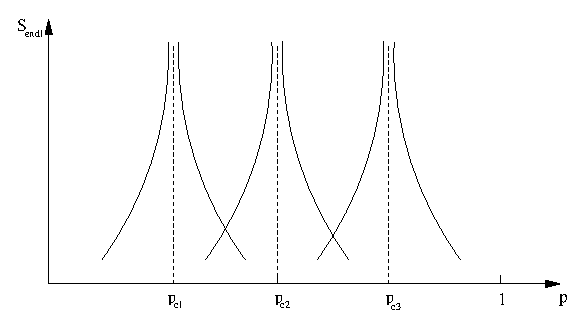
\includegraphics{./Einleitung-figs/universal}
  \caption{Schematische Darstellung des universellen asymptotischen Verhalten der mittleren Clustergr\"o"se endlicher Cluster $S_{endl}(p)$ von Perkolationsprozessen mit unterschiedlichem $p_c$.}
  \label{fig:universal}
\end{figure}
\\Der Perkolationsprozess ist in vielen Aspekten kontinuierlichen thermischen Phasen\"uber\-g\"an\-gen mit divergierender Korrelationsl\"ange sehr \"ahnlich. In der Tat geht der Phasen\"ubergang in Spinmodellen mit dem erstmaligen Auftreten eines unendlichen Spinclusters einher \cite{Coniglio:77}. Perkolation kann als Limes $\lambda \rightarrow 1$ des $\lambda$-Zustands-Pottsmodells erhalten werden (\cite{Fortuin:72}, siehe auch Abschnitt \ref{sec:matchingpoly}). $P_{\infty}(p)$ spielt die Rolle des Ordnungsparameters, die mittlere Clustergr\"o"se $S$ die der Suszeptibilit\"at und die charakteristische L\"ange der Pair-connectedness Funktion entspricht der Korrelationsl\"ange zweier Spins.\\
Perkolation wurde als Modell f\"ur ungeordnete por\"ose Medien eingef\"uhrt und hat im Laufe der Jahrzehnte in so unterschiedlichen Bereichen wie Epidemologie, der Theorie der Phasen\"uberg\"ange und der Beschreibung kosmischer Strukturen Anwendungen gefunden. F\"ur eine umfassende Einf\"uhrung in die mathematische Perkolationstheorie sei auf die B\"ucher von Grimmett \cite{Grimmett:99} und Hughes \cite{Hughes:96} verwiesen, f\"ur die physikalischen Aspekte der Perkolationstheorie ist das Buch von Stauffer und Aharony \cite{Stauffer:95} eine unterhaltsame Quelle.\\

Das Hauptaugenmerk der Perkolationstheorie liegt auf dem Verst\"andnis der universellen Eigenschaften in der N\"ahe des kritischen Punktes. F\"ur viele praktische Anwendungen ist aber die Kenntnis des Wertes von $p_c$ entscheidend. Die Art und Weise, wie $p_c$ von den mikroskopischen Details des Perkolationsprozesses, insbesondere der Gitterstruktur abh\"angt, ist Gegenstand dieser Arbeit. Klaus Mecke und Herbert Wagner haben bemerkt, dass die Nullstelle $p_0$ der mittleren Euler-Charakteristik bei einer Reihe von Perkolationsproblemen in der N\"ahe von $p_c$ liegt. Das Ziel der Arbeit ist es, diesen Befund ausf\"uhrlicher zu untersuchen, und $p_0$ als Sch\"atzwert f\"ur $p_c$ empirisch zu begr\"unden. Diese Faustregel ist vergleichbar mit dem Lindemann-Kriterium f\"ur das Schmelzen von Kristallen, welches besagt, dass ein Kristall schmilzt, sobald die mittlere Schwingungsamplitude der Kristall\-atome ungef\"ahr $1/10$ des Gitterabstandes erreicht. In vergleichbarer Weise ist die Nullstelle der Euler-Charakteristik geeignet den Perkolations\"ubergang abzusch\"atzen. In zwei Dimensionen ist die Euler-Charakteristik die Differenz der Zahl der Cluster und der Zahl der in diesen Clustern enthaltenen L\"ocher. Die Euler-Charakteristik wird negativ, wenn die L\"ocher \"uberwiegen. Unterhalb von $p_c$ besteht die Anordnung aus vielen endlichen Clustern, die L\"ocher enthalten k\"onnen. Oberhalb von $p_c$ exisitert ein unendlicher Cluster, der unbesetzte Inseln enth\"alt, die wiederum endliche besetzte Cluster enthalten k\"onnen. Oberhalb von $p_c$ ist also jeder endliche Cluster in einem Loch des unendlichen Clusters enthalten und jeder positive Beitrag zur Euler-Charakteristik geht mit einem negativen Beitrag einher. Man erwartet also f\"ur $p<p_c$ positive und f\"ur $p>p_c$ negative Euler-Charakteristik und es ist plausibel, dass $p_0$ in der N\"ahe von $p_c$ liegt. 

\subsection{Weitere Perkolationsmodelle}
Als anschauliche Beispiele f\"ur bond- und site-Perkolation haben wir Saboteure betrachtet, die in zuf\"alliger Reihenfolge entweder Verbindungen oder Knoten eines Netzwerkes zerst\"oren. Wenn zwei verschiedene Gruppen von Saboteuren, von denen eine Verbindungen und die andere Knoten zerst\"ort, gleichzeitig eine Attacke starten, erzeugen sie einen gemischten \textbf{bond-site-Perkolationsprozess}. Die Bruchteile der Verbindungen $p_b^*$ und Knoten $p_s^*$, die zum Zeitpunkt, an dem die Leitf\"ahigkeit verschwindet, zerst\"ort sind, h\"angen von den Geschwindigkeiten ab, mit denen Verbindungen bzw. Knoten zerst\"ort werden. Der kritische Ort ist eine Kurve $p_s^*(p_b^*)$ in der $(p_s,p_b)$-Ebene. Auch die anderen angef\"uhrten Beispiele lassen sich leicht auf bond-site-Perkolation verallgemeinern. Wenn beim Modell der Gelierung nur auf einem Bruchteil der Gitterpunkte ein Monomer sitzt, erh\"alt man einen bond-site-Perkolationsprozess. Entsprechend k\"onnten im Waldbrandmodell brennende B\"aume ihre Nachbarn nicht mit Sicherheit, sondern nur mit einer gewissen Wahrscheinlichkeit entz\"unden.\\
Perkolation auf Gittern ist ein einfaches Modell, das reale Ph\"anomene nur eingeschr\"ankt wiedergeben kann. Perkolation kann aber ebenso gut als kontinuierliches Modell formuliert werden. Man kann beispielsweise Punkte nach einen gewissen Zufallsprozess verteilen und sie nach einer geeigneten Vorschrift als verbunden einstufen. Das prominenteste Modell ist das Boolsche Kornmodell. Man betrachtet poissonverteilte Punkte und heftet an diese Punkte geometrische K\"orper. \"Uberlappen die K\"orper, sind die entsprechenden Punkte verbunden. Ab einer gewissen Punktdichte tritt ein unendlicher Cluster auf. Verschiedene Perkolationsmodelle im Kontinuum sind im Buch von Meester und Roy \cite{Meester:96} ausf\"uhrlich beschrieben. Viele mathematische Resultate f\"ur Perkolation auf Gittern gelten in analoger Weise auch f\"ur Kontinuumsperkolation. \\
In allen bisher diskutierten F\"allen wurden Verbindungen bzw. Vertices unabh\"angig voneinander ge\"offnet bzw. besetzt. Es gibt auch Modelle, in denen die Konstituenten miteinander wechselwirken und die Verteilung der ge\"offneten Verbindungen bzw. besetzten Vertices Korrelationen aufweist. Ein prototypisches Beispiel sind Cluster gleich ausgerichteter Spins in den Spinmodellen des Ferromagnetismus. Benachbarte Spins wechselwirken miteinander, und wir bezeichen die Verbindung zwischen zwei benachbarten Spins als ge\"offnet, wenn sie parallel ausgerichtet sind. Dadurch entsteht ein Perkolationsprozess, in dem Verbindungen nicht unabh\"angig voneinander ge\"offnet sind. Ohne \"au"seres Feld richten sich isolierte Cluster unabh\"angig voneinander aus und der Betrag des Erwartungswertes der Magnetisierung ist null. Wenn die Spincluster perkolieren, existiert ein einziger unendlicher Cluster und die Magnetisierung ist von null verschieden. Der Perkolations\"ubergang der Spincluster f\"allt also mit dem thermischen Phasen\"ubergang zusammen \cite{Coniglio:77}.\\
Ein weitere interessante Anwendung der Perkolationstheorie sind verd\"unnte Isingmodelle. Werden in einem Gitter von Spins mit ferromagnetischer Wechselwirkung mit Wahrscheinlichkeit $q$ Leerstellen eingef\"ugt, sinkt die kritische Temperatur $T_c$. Wenn $q$ so gro"s wird, dass $p=1-q<p_c$ ist, zerf\"allt das Spingitter in endliche Cluster und es kann kein Phasen\"ubergang mehr auftreten. $T=0$ und $p=1-q=p_c$ ist ein multikritscher Punkt, an dem sowohl die thermische Korrelationsl\"ange der Spins $\xi_T$, als auch die L\"angenskala $\xi_P$ der pair-connectedness Funktion $\rho(r)$ divergieren. In Abbildung \ref{fig:diluted} sind der Verlauf von $T_c(p)$ und das verd\"unnte Isingmodell skizziert.
\begin{figure}[tbp]
  \centering
  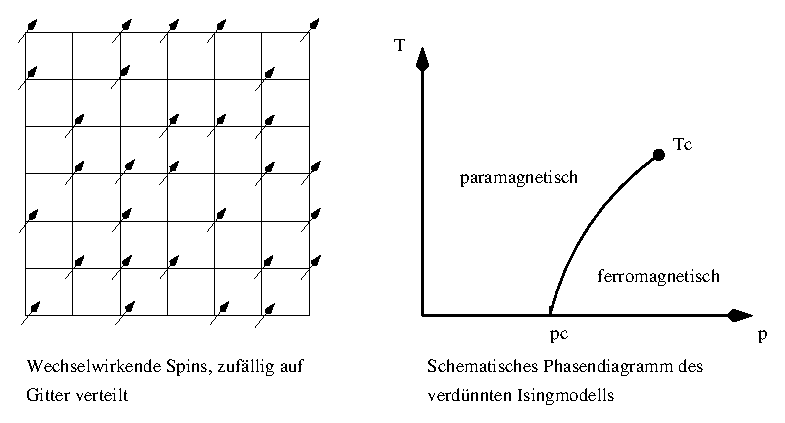
\includegraphics{./Einleitung-figs/diluted}
  \caption{Verd\"unntes Isingmodell}
  \label{fig:diluted}
\end{figure}

\section{Clusterzahlen}
Bei einem Perkolationsprozess auf einem Gitter entstehen in zuf\"alliger Weise zusammenh\"ang\-ende Bereiche. Zwei besetzte Vertices des Gitters sind verbunden, wenn sie n\"achste Nachbarn sind und die Gitterkante zwischen ihnen ge\"offnet ist. Eine maximale Menge von Vertices, die untereinander durch eine Kette von Vertices verbunden sind, hei"st Cluster. Wenn die Verteilung der Cluster bekannt ist, k\"onnen alle f\"ur die Perkolationstheorie relevanten Gr\"o"sen ausgerechnet werden.
\subsection{site-Perkolation in einer Dimension}
Auf einer eindimensionalen Kette von Vertices sind die einzigen m\"oglichen Cluster zusammenh\"angende St\"ucke der Kette. Jeder Cluster ist durch seine L\"ange vollst\"andig festgelegt. 
\begin{figure}[bp]
  \centering
  \includegraphics{./Einleitung-figs/1d_simple}
  \caption{Kette von unbesetzten und besetzten Vertices. Es treten Cluster der Gr\"o"sen 1, 3 und 4 auf. Die Wahrscheinlichkeit dieser Anordnung ist $qpqqpppqppppq=p^8q^5$ ($q=1-p$). }
  \label{fig:1d_simple}
\end{figure}
Damit ein Vertex das linke Ende eines Clusters der Gr\"o"se $s$ ist, muss sein linker Nachbar unbesetzt, er selbst und seine $s-1$ rechten Nachbarn besetzt, und der darauffolgende Vertex wiederum unbesetzt sein (siehe Abb. \ref{fig:1d_simple}). Die Wahrscheinlichkeit dieses Ereignisses ist $n_s(p)=p^s(1-p)^2$. $n_s$ ist die erwartete Anzahl der Cluster der Gr\"o"se $s$ pro Vertex. Summiert man \"uber alle $s$, erh\"alt man die Gesamtzahl der Cluster pro Vertex
\begin{equation}
  n(p)=(1-p)^2\sum_{s=1}^\infty p^s=p(1-p).
\end{equation}
Ein besetzter Vertex ist unterhalb von $p_c$ in genau einem endlichen Cluster enthalten. Der Vertex kann an jedem der $s$ Pl\"atze eines Clusters der Gr\"o"se $s$ sein und die bedingte Wahrscheinlichkeit f\"ur dieses Ereignis ist $\mathcal{P}\{ x\in \text{Cluster der Gr\"o"se} \; s\:|\: x \; \text{ist besetzt}\}=sp^{s-1}(1-p)^2$. Jeder Vertex ist mit Wahrscheinlichkeit $p$ besetzt und es gilt\begin{equation}
  p=(1-p)^2\sum_{s=1}^\infty sp^s.
\end{equation}
Die mittlere Gr\"o"se des Clusters, zu dem ein beliebiger besetzter Vertex geh\"ort, ist durch
\begin{equation}
  S=\frac{(1-p)^2}{p}\sum_{s=1}^\infty s^2p^s=\frac{p+1}{p-1}
\end{equation}
gegeben. Die mittlere Clustergr\"o"se ist f\"ur $p<1$ endlich und divergiert im Limes vollst\"andiger Besetzung. Die Wahrscheinlichkeit, dass ein Vertex Teil eines Clusters der Gr\"o"se $s$ ist, ist f\"ur $p<1$ proportional zu $sp^s$. Im Limes unendlicher Clustergr\"o"se gilt
\begin{equation}
\lim_{s\rightarrow{\infty}} sn_s(p)= \begin{cases} 0 \qquad \text{f\"ur} \qquad p<1, \\ 1 \qquad \text{f\"ur} \qquad p=1. \end{cases}
\end{equation}
Daher ist in einer Dimension die triviale Perkolationsschwelle $p_c=1$, und es gibt keine perkolierende Phase. Die Euler-Charakteristik einer eindimensionalen Figur ist gleich der Zahl der Komponenten. Die mittlere Euler-Charakteristik pro Vertex is also $\chi(p)=n(p)=p(1-p)$. Ihre Nullstelle $p_0=1$ f\"allt mit $p_c$ zusammen.\\
Auch auf einem zweidimensionalen Gitterstreifen mit unendlicher Ausdehnung in horizontaler Richtung und endlicher H\"ohe $l$ tritt f\"ur $p<1$ kein unendlicher Cluster auf (siehe Abb. \ref{fig:1D}). Die Wahrscheinlichkeit, dass zwischen oberen und unteren Rand eine senkrechte Kette unbesetzter Gitterpl\"atzen exisitiert, ist $Q=(1-p)^l>0$. Damit ein Cluster eine horizontale L\"ange $s$ hat, d\"urfen an $s$ Stellen keine solchen Ketten auftreten. Daher ist die Wahrscheinlichkeit, dass ein Cluster mit horizontaler Ausdehnung $s$ auftritt, kleiner als $(1-Q)^s$ und verschwindet f\"ur gro"se $s$. \\
\begin{figure}[htbp]
  \centering
  \includegraphics{./Einleitung-figs/1D}
  \caption{Cluster mit Ausdehnung $s$ auf einem Gitterstreifen der H\"ohe $l=5$; die Verbindungen von oben nach unten aus unbesetzten Gitterpl\"atzen sind in grau dargestellt. }
  \label{fig:1D}
\end{figure}
\subsection{Clusterzahlen in zwei Dimensionen}
\label{sec:animals}
W\"ahrend in einer Dimension ein Cluster nur durch seine L\"ange eindeutig beschrieben werden konnte, k\"onnen in zwei Dimensionen aus $s$ Vertices i. A. viele verschiedene Cluster gebildet werden. Damit ein bestimmter Cluster auftritt, m\"ussen alle Vertices, die zu ihm geh\"oren, besetzt und die umgebenden Vertices unbesetzt sein. Die Wahrscheinlichkeit, dass ein bestimmter Cluster auftritt, h\"angt also von seiner Masse $s$ und der L\"ange seines ``Perimeters'' $t$ ab und ist durch $p^s(1-p)^t$ gegeben. Cluster des Quadratgitters bis zur Masse $s=3$ sind in Abb. \ref{fig:2d_cluster} gezeigt. 
\begin{figure}[tbp]
  \centering
  \includegraphics{./Einleitung-figs/2D_cluster}
  \caption{Cluster des Quadratgitters bis zur Masse $s=3$.}
  \label{fig:2d_cluster}
\end{figure}
Die erwartete Zahl der Cluster der Gr\"o"se $s$ pro Vertex ist mit $q=1-p$ f\"ur $s=1,2,3$
\begin{eqnarray}
n_1(p) & = & pq^4, \\
n_2(p) & = & 2p^2q^6, \\
n_3(p) & = & 2p^3q^8+4p^3q^7,
\end{eqnarray}
und allgemein
\begin{equation}
n_s(p)=\sum_t g_{st}p^sq^t=p^sD_s(p).
\end{equation}
Hierbei sind $g_{st}$ die Zahlen der Cluster der Masse $s$ und Umfangsl\"ange $t$. $D_s(p)=\sum_t g_{st}q^t$ sind die sogenannten Perimeterpolynome. Die Zahlen $g_{st}$ sind f\"ur verschiedene Gitter bis $s$ in der Gr\"o"senordnung von 20 mit Computern abgez\"ahlt worden. Bond-Perkolation kann auf dem \"Uberdeckungsgitter ganz analog als site-Perkolation behandelt werden.\\
Man kann die Cluster erzeugen, indem man, ausgehend von einem einzigen besetzten Vertex, sukzessive am Perimeter weitere Vertices besetzt. Dieser Prozess \"ahnelt der Vermehrung eines Zellhaufens durch Zellteilung. Daher werden diese Cluster oft \textbf{lattice animals} oder \textbf{Gittertiere} genannt.\\
Ein bestimmter besetzter Vertex kann jeder der $s$ Vertices eines Clusters der Masse $s$ sein und ist daher mit Wahrscheinlichkeit $sn_s(p)$ Teil eines solchen Clusters. Unterhalb von $p_c$ geh\"ort jeder besetzte Vertex zu einem endlichen Cluster, und da jeder Vertex mit Wahrscheinlichkeit $p$ besetzt ist, gilt
\begin{equation}
p=\sum_{s}sn_s(p) \qquad \text{f\"ur}\qquad p<p_c.
\end{equation}
In der perkolierenden Phase ist ein besetzter Vertex mit Wahrscheinlichkeit $P_\infty(p)$ Teil des unendlichen Cluster, und daher gilt
\begin{equation}
p=\sum_{s}sn_s(p)+P_\infty(p).
\end{equation}
Die mittlere Gr\"o"se der endlichen Cluster erh\"alt man in Analogie zum eindimensionalen Fall durch
 \begin{equation}
S_{endl}(p)=\frac{1}{p}\sum_{s}s^2n_s(p).
\end{equation}
Clusterzahlen in h\"oheren Dimensionen werden ganz analog zu denen in zwei Dimensionen definiert.

\subsection{Perkolation auf dem Bethe-Gitter}
Auf dem Bethe-Gitter l\"asst sich das Perkolationsproblem geschlossen l\"osen. Das Bethe-Gitter hat keine geschlossenen Schleifen, und zwischen zwei Vertices existiert \textbf{genau} eine Kette von Vertices, die beide Vertices verbindet. Die eindimensionale Kette ist ein spezielles Bethe-Gitters.
\begin{figure}[tbp]
  \centering
  \includegraphics{./Einleitung-figs/bethe}
  \caption{Ein kleiner Auschnitt eines Bethe-Gitters mit $z=3$. Das Gitter l\"asst sich in Schalen $n=1,2,3,\ldots$ um den Ursprung zerlegen. }
  \label{fig:caley}
\end{figure}
\\Von einem Vertex des Bethe-Gitters gehen $z$ Verbindungen zu $z$ anderen Vertices, von diesen $z-1$ weitere Verbindungen zu neuen Vertices usw. (siehe Abb. \ref{fig:caley}). Von jedem Vertex gehen also $z$ \"Aste aus und der einzige gemeinsame Vertex dieser \"Aste ist der Ursprungsvertex. Dieser Vertex hat $z$ n\"achste Nachbarn, $z(z-1)$ \"ubern\"achste Nachbarn und $z(z-1)^{n-1}$ Vertices, die $n$ Schritte entfernt sind. Wir betrachten wiederum site-Perkolation und besetzen Vertices mit Wahrscheinlichkeit $p$.  Da zwei Vertices durch \textbf{genau} eine Kette von Vertices miteinander verbunden sind, ist die Wahrscheinlichkeit, dass zwei $n$ Schritte entfernte Vertices besetzt und verbunden sind durch $p^{n+1}$ gegeben. Es gibt gerade $z(z-1)^{n-1}$ $n$ Schritte entfernte Vertices und ein willk\"urlich ausgezeichneter Ursprung ist im Mittel mit $N_n=\frac{pz}{z-1}[p(z-1)]^n$ Vertices im Abstand $n$ verbunden. Gilt $p>\frac{1}{z-1}$, ist die Wahrscheinlichkeit, dass der Ursprung mit beliebig weit entfernten Vertices verbunden ist, gr\"o"ser $0$; ist $p<\frac{1}{z-1}$ verschwindet $N_n$ exponentiell mit $n$. Die Perkolationsschwelle liegt also bei $p_c=\frac{1}{z-1}$. Die mittlere Clustergr\"o"se erh\"alt man f\"ur $p(z-1)<1$ durch Summation der $N_n$ \"uber $n$
\begin{equation}
  \begin{split}
  S & = p+\frac{pz}{z-1}\sum_{n=1}^{\infty}[p(z-1)]^{n}=p+\frac{pz}{z-1}\left[\frac{1}{1-p(z-1)}-1\right] \\
  & =\frac{p(p+1)}{1-p(z-1)}=\frac{p_cp(1+p)}{p_c-p}.
\end{split}
\end{equation}
Die mittlere Clustergr\"o"se divergiert f\"ur $p\rightarrow p_c$ wie $S\sim \frac{1}{p_c-p}$. Der kritische Exponent $\gamma$ hat also den Wert 1. Auch die \"ubrigen Exponenten k\"onnen analog bestimmt werden, und man erh\"alt $\beta=1$ und $\nu=1/2$.\\ 
Die Zahl der Vertices, die weniger als $N+1$ Schritte vom Ursprung entfernt sind, ist f\"ur $z>2$ gleich $V=1+z\sum_{n=0}^{N-1}(z-1)^n=(z-1)^N$. Die Zahl der Vertices, die genau $N$ Schritte vom Ursprung entfernt sind, ist $A=z(z-1)^{N-1}$. $V$ und $A$ entsprechen dem Volumen und der Oberfl\"ache einer Kugel mit Radius $N$. In \"ublichen $d$-dimensionalen Gittern verh\"alt sich Kugeloberfl\"ache zu Kugelvolumen wie $A \sim V^{1-1/d}$. F\"ur gro"se $d$ sind Oberf\"ache und Volumen also fast proportional zueinander. Daher kann das Bethe-Gitter mit $z>2$ als Modell f\"ur Gitter hoher Dimension aufgefasst werden. Tats\"achlich stimmen die kritischen Exponenten der Perkolation auf dem Bethe-Gitter mit denen auf Gittern mit $d>19$ \"uberein. Vermutlich gilt diese \"Ubereinstimmung sogar herab bis $d=6$. F\"ur $z=2$ wird der eindimensionale Fall reproduziert. \\
Bond-Perkolation wird ganz analog behandelt und man erh\"alt die gleiche Perkolationsschwelle.\\  
Die Euler-Charakteristik eines Baumgraphen ist (zur Euler-Charakteristik siehe Kapitel \ref{sec:Euler}) die Differenz der Zahl der Vertices und Kanten. Betrachtet man die Vertices und Kanten innerhalb von $N$ Schalen um den Ursprung, kann die mittlere Euler-Charakteristik des Graphens in diesem Beobachtungsfenster bestimmt werden. Bei der site-Perkolation werden Vertices mit Wahrscheinlichkeit $p$ besetzt und eine Kante zwischen zwei Vertices ist mit Wahrscheinlichkeit $p^2$ vorhanden. Entsprechend sind bei bond-Perkolation alle Vertices besetzt, und Kanten sind mit Wahrscheinlichkeit $p$ vorhanden. Beide F\"alle unterscheiden sich also nur durch einen Faktor $p$. F\"ur die Euler-Charakteristik bei site-Perkolation ergibt sich
\begin{equation}
  \chi^{site}_N(p)=p\left[1+z\sum_{n=1}^N(z-1)^{n-1}\right]-p^2\left[z\sum_{n=1}^{N+1}(z-1)^{n-1}\right].
\end{equation}
Hierbei wurden alle Kanten, die aus dem Beobachtungsfenster hinausf\"uhren, mitgez\"ahlt. Die Nullstelle $p_0$ konvergiert f\"ur $N\rightarrow \infty$ gegen $\frac{1}{z-1}$. Das gleiche Resultat gilt im Fall der bond-Perkolation. Wie bei Perkolation in einer Dimension, stimmt $p_0$ mit $p_c$ auf dem Bethe-Gitter \"uberein.\\ 

\section{Perkolationsschwellen}

Nachdem Perkolation in groben Z\"ugen vorgestellt wurde, wird im Folgenden Bekanntes zu Perkolationsschwellen zusammengetragen. 

\subsection{Rigorose Ungleichungen}
Im Allgemeinen sind f\"ur Perkolationsschwellen nur sehr grobe Ungleichungen bekannt. Nichttriviale, allgemein g\"ultige Ungleichungen sind $p_c^{site}\geq p_c^{bond}$ und $p_c^{bond}\geq \frac{1}{\mu} \geq \frac{1}{z-1}$, wobei $\mu$ die Konnektivit\"atszahl und $z$ die Koordinationszahl des betrachteten Gitters ist. Die Konnektivit\"atszahl ist durch $\mu=\lim_{n\rightarrow \infty}\frac{\ln N_{SAW}^n}{n}$ definiert, wobei $N_{SAW}^n$ die Zahl der selbstvermeidenden Wege der L\"ange $n$ auf dem betrachteten Gitter ist. In zwei Dimensionen folgt aus der matching-Eigenschaft (siehe unten) eine obere Schranke an $p_c^{site}$. Da Gitter der Dimension $d$ perkolieren, wenn $(d-1)$-dimensionale Untergitter perkolieren, k\"onnen Perkolationschwellen mit $d$ h\"ochstens abnehmen, sind aber echt gr\"o"ser als $0$. F\"ur alle Gitter mit $d \geq 2$ gilt also $0 < p_c^{bond} \leq p_c^{site}<1$. Auf allen Gittern in $d\geq 2$ existiert daher eine nicht perkolierende Phase $p<p_c$ und einen Bereich $p>p_c$, in dem ein unendlicher Cluster exisitert. Auf einige Gitter, deren Perkolationsschwellen exakt bekannt sind, wird im Kapitel \ref{sec:dualitaet} genauer eingegegangen. F\"ur site-Perkolation auf dem Quadrat-, dice- und Sechseckgitter, sowie f\"ur bond-Perkolation auf dem Kagom\'egitter existieren rigorose obere und untere Schranken f\"ur die Perkolationschwellen. Diese Schranken und die zugeh\"origen Referenzen sind Referenz \cite{Hughes:96} entnommen. 
\begin{eqnarray}
& 0.5416\leq p_c^{sq-site}\leq0.6795 & \quad \text{Wierman \cite{Wierman:95}, Men'shikov und Pelikh \cite{Menshikov:89}}\\
& p_c^{hex-bond}\leq p_c^{hex-site}\leq 0.8079  &\quad \text{Luczak und Wiermann \cite{Luczak:88}}\\
& 0.5182 \leq p_c^{kag-bond}\leq 0.5335 & \quad \text{Wierman \cite{Wierman:90}}\\
& 0.520 \leq p_c^{dice-site}\leq 0.7937 &\quad \text{Luczak und Wiermann \cite{Luczak:88}}
\end{eqnarray}
Um diese Schranken herzuleiten, ist erheblicher mathematischer Aufwand n\"otig. Dar\"uberhinaus sind wenig rigorose Resultate \"uber Perkolationsschwellen bekannt.  


\subsection{Dualit\"at und matching -- exakte Perkolationsschwellen}
\label{sec:dualitaet}
In zwei Dimensionen sind einige Perkolationsschwellen exakt bekannt. Die exakte Bestimmung der Perkolationsschwellen beruht auf der Tatsache, dass es zu jedem zweidimensionalen Gitter ein sog. \textit{duales Gitter} gibt, und die Perkolationsschwellen dieser beiden Gittern miteinander in Verbindung gebracht werden k\"onnen. 
\\Ein planarer Graph $G$ l\"asst sich in die Ebene einbetten, ohne dass sich zwei Kanten schneiden (f\"ur eine Definition dieser Begriffe siehe \ref{sec:graphen} oder \cite{Essam:70}). Der Graph zerschneidet die Ebene in endliche Gebiete. Setzt man in jedes dieser endlichen Gebiete und in das Gebiet au"serhalb des Graphens einen Vertex und verbindet Vertices, deren Gebiete sich an einer Kante von $G$ ber\"uhren, erh\"alt man den dualen Graphen $G^*$ (siehe Abb. \ref{fig:dualgraph}).
\begin{figure}[htbp]
  \centering
  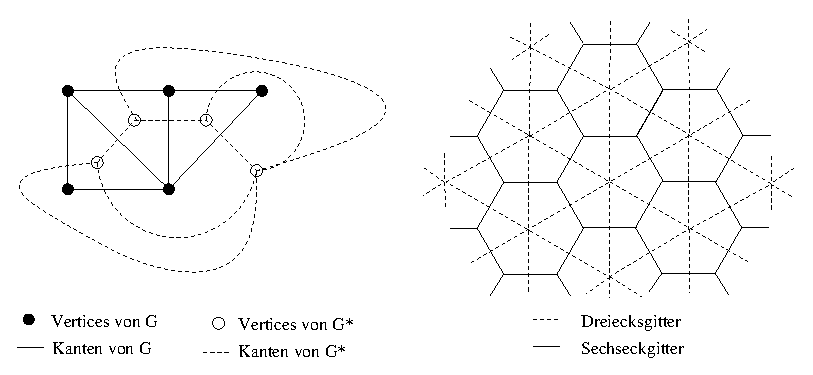
\includegraphics{./Einleitung-figs/dualgraph}
  \caption{Links: Jede Kante des Graphen $G$ wird von einer Kante des dualen Graph $G^*$ geschnitten. Rechts: Das Dreiecks- und Sechseckgitter bilden ein Paar dualer Gitter.}
  \label{fig:dualgraph}
\end{figure}
Die Dualit\"atstransformation stiftet eine eins-zu-eins-\-Korrespondenz zwischen den Kanten des Graphen und denen des dualen Graphens. Zweidimensionale Gitter sind periodisch fortgesetzte Graphen und zu jedem Gitter $\mathcal{G}$ kann ein duales Gitter $\mathcal{G}^*$ konstruiert werden. Wir interessieren uns f\"ur Paare dualer Gitter. Jede Kante in $\mathcal{G}^*$ schneidet genau eine Kante in $\mathcal{G}$ und die Kantenmengen $E$ und $E^*$ von $\mathcal{G}$ und $\mathcal{G}^*$ k\"onnen identifiziert werden. Ihre Vertexmengen $V$ und $V^*$ sind aber i. A. unterschiedlich.\\
Wir betrachten nun bond-Perkolation auf $\mathcal{G}$ und besetzen einen Teil der Kanten $E'\subset E$ von $\mathcal{G}$. Es entsteht eine Subgraph $G$ mit Vertexmenge $V$ und Kantenmenge $E'$. Da jede Kante aus $\mathcal{G}$ eine Kante aus $\mathcal{G}^*$ schneidet, betrachten wir nun den Subgraph $G^*$ von $\mathcal{G}^*$ mit Vertexmenge $V^*$ und Kantenmenge $E^{*'}=E\backslash E'$. Die Komponenten von $G$ bzw. $G^*$ sind Cluster auf den Gittern $\mathcal{G}$ bzw. $\mathcal{G}^*$. Jeder endliche Cluster auf $\mathcal{G}$ ist von einem Cluster auf $\mathcal{G}^*$ umschlossen, denn alle unbesetzten Kanten am Rand eines Clusters werden von besetzten dualen Kanten geschnitten. Umgekehrt gilt dasselbe (siehe Abb. \ref{fig:dual}). Betrachtet man einen gro"sen rechteckigen Ausschnitt des Gitters, so existiert ein Cluster auf $\mathcal{G}$, der den linken und rechten Rand des Rechtecks verbindet, genau dann, wenn kein solcher Cluster auf $\mathcal{G}^*$ den oberen und unteren Rand verbindet. Besetzt man Kanten von $\mathcal{G}$ mit Wahrscheinlichkeit $p$, so entsteht ein komplement\"ares Perkolationsproblem mit Besetztungswahrscheinlichkeit $q=1-p$ auf $\mathcal{G}^*$. F\"ur die Perkolationschwellen gilt 
\begin{equation}
  p_c^{bond}(\mathcal{G})+p_c^{bond}(\mathcal{G}^*)=1.
\end{equation}
Das Quadratgitter ist ``selbstdual'' und $p_c=\frac{1}{2}$ (siehe Abb. \ref{fig:dual}). Das Dreiecks- und das Sechseckgitter sind ein duales Paar und k\"onnen durch die sogenannte Stern-Dreiecks-Transformation ineinander \"uberf\"uhrt werden. Dadurch erh\"alt man f\"ur $p_c$ eine zus\"atzliche Gleichung und die L\"osung $p_c^{Dreieck}=1-p_c^{Sechseck}=2\sin(\pi/18)$. Diese \"Uberlegungen gehen auf Sykes und Essam \cite{Sykes:64} zur\"uck, sind aber nicht im mathematischen Sinne rigoros. Wierman \cite{Wierman:84} hat eine verallgemeinerte Stern-Dreieckstransformation auf das bowtie-Gitter angewendet. Die bond-Perkolationsschwelle $p_c$ ist die L\"osung von $1-p-6p+6p^3-p^5=0$ und hat den numerischen Wert $p_c=0.404518\ldots$.
\begin{figure}[htbp]
  \centering
  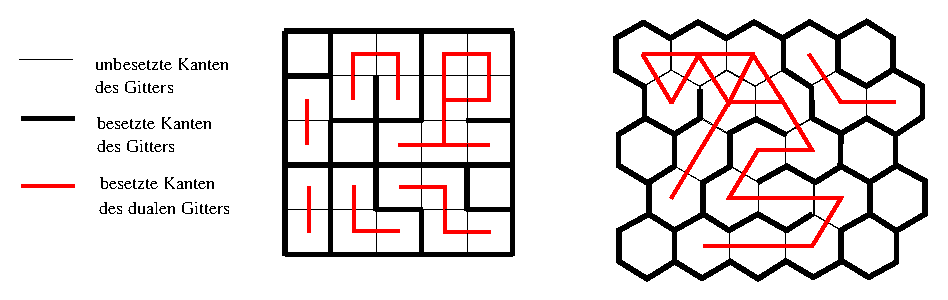
\includegraphics{./Einleitung-figs/dualnew}
  \caption{Komplement\"are Besetzung der Kanten eines Paares dualer Gitter am Beispiel des selbstdualen Quadratgitters und des Dreiecks- und Sechseckgitters.}
  \label{fig:dual}
\end{figure}
\\Jedem bond-Perkolationsproblem entspricht ein site-Perkolationsproblem auf dem \"Uberdeckungsgitter (siehe Abb. \ref{fig:covering_einleit}). Also sollte sich die Dualit\"ats-Eigenschaft auf die site-Perkolation \"ubertragen lassen. Dies ist in der Tat m\"oglich, allerdings muss der Gitterbegriff auf nichtplanare Gitter, sog. ``dekorierte Mosaike'', verallgemeinert werden. Man geht von einem planaren Gitter, im folgenden \textit{Mosaik} genannt, aus und erg\"anzt bei einem Teil der Plaketten alle diagonalen Verbindungen. Eine solche Plakette hei"st \textit{dekoriert} und das resultierende, im Allgemeinen nicht mehr planare, Gitter \textit{dekoriertes Mosaik}. Das matching-Gitter  $\mathcal{G}^+$ zu einem dekorierten Mosaik $\mathcal{G}$ erh\"alt man, indem das Mosaik komplement\"ar dekoriert wird, d.h. die Plaketten die in $\mathcal{G}$ nicht dekoriert waren, werden in $\mathcal{G}^+$ dekoriert und umgekehrt (siehe Abb. \ref{fig:matchinggitter}). 
\begin{figure}[tbp]
  \centering
  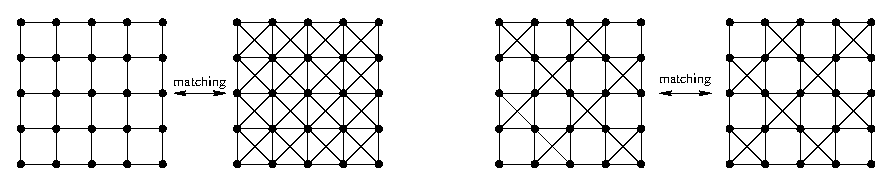
\includegraphics{./Einleitung-figs/matchinggitter}
  \caption{Links: Ein Vertex des Quadratgitters hat vier n\"achste Nachbarn, einer des matching-Gitters acht. Rechts: Die Gitter sind selfmatching. Sie sind das \"Uberdeckungsgitter des Quadratgitters.}
  \label{fig:matchinggitter}
\end{figure}
$\mathcal{G}=(V,E)$ und $\mathcal{G}^+=(V,E^+)$ haben die gleiche Vertexmenge, aber i. A. unterschiedliche Kantenmengen. Die Kanten des Mosaiks sind in $E$ und $E^+$ enthalten. Die Graphen $G$ und $G^+$ mit Vertexmengen $I \subset V$ und $I^+=V \backslash I$ und Kantenmengen $K=\{x,y\in I|xy \in E\}$ und $K^+=\{x,y\in I^+|xy \in E^+\}$ haben die entsprechende Dualit\"atseigenschaft: Jede endliche Komponente von $G$ ist in einem geschlossenen Weg in $G^+$ enthalten; dies gilt in analoger Weise umgekehrt (siehe Abb. \ref{fig:matching}). Die site-Perkolationsschwellen zweier matching-Gitter erg\"anzen sich zu 1. Aus der matching-Eigenschaft kann man einfach eine nichtriviale obere Schranke an die site-Perkolationsschwelle gewinnen, denn $p_c^{site}(\mathcal{G})=1-p_c^{site}(\mathcal{G}^+) \leq 1-\frac{1}{\mu^+}\leq 1-\frac{1}{z^+-1}<1$.\\
Das Dreiecksgitter ist selfmatching, denn alle Ecken eines Dreiecks sind Nachbarn, und es gibt keine Verbindungen, die erg\"anzt werden k\"onnten. Daher ist die site-Perkolationsschwelle des Dreiecksgitters $p_c=\frac{1}{2}$. Im matching-Gitter eines planaren Gitters sind alle Plaketten dekoriert und daher alle Vertices auf dem Rand einer Plakette n\"achste Nachbarn (siehe linker Teil in Abb. \ref{fig:matchinggitter}). Ein planares Gitter ist immer ein Subgraph seines matching-Gitters und hat daher eine h\"ohere Perkolationsschwelle als sein matching-Gitter. Daher ist $p_c^{site} \geq \frac{1}{2}$ f\"ur alle planaren Gitter.
Das Kagom\'e-Gitter ist das \"Uberdeckungsgitter des Sechseckgitters, und es gilt $p_c^{site-Kagome}=p_c^{bond-Sechseck}$. \\
\begin{figure}[htbp]
  \centering
  \includegraphics{./Einleitung-figs/match}
  \caption{Komplement\"ar besetzte Paare von matching-Gittern am Beispiel des Quadrat- und Dreiecksgitters.}
  \label{fig:matching} 
\end{figure}


\subsection{Empirische Formeln f\"ur Perkolationsschwellen}
In Literatur \"uber Perkolation sind des \"ofteren empirische Formeln f\"ur Perkolationsschwellen in Abh\"angigkeit von Koordinationszahl $z$ und Dimension $d$ vorgestellt worden. F\"ur bond-Perkolation gilt in zwei Dimensionen als grobe N\"aherung $p_c\approx \frac{2}{z}$, f\"ur hoch-dimensionale Gitter $p_c \approx \frac{1}{z-1}$. Andere Formeln enthalten eine Reihe von Fitparametern und sagen $p_c$ als Funktion von $d$ und $z$ voraus. Tats\"achlich variieren Perkolationsschwellen auf Gittern der gleichen Dimension und gleicher Koordinationszahl betr\"achtlich, so dass eine Vorhersage von Perkolationsschwellen allein aus $d$ und $z$ nicht sinnvoll erscheint. \\
Scher und Zallen \cite{Scher:70} beobachteten einen Zusammenhang zwischen site-Perkolationsschwel\-len und der Packungsdichte $f$ f\"ur zwei- und dreidimensionale Gitter. Die Packungsdichte ist der Anteil des Raums (Ebene), der bedeckt ist, wenn auf jeden Vertex des Gitters eine Kugel (Kreisscheibe) mit Radius der halben Kantenl\"ange sitzt. F\"ur das \mbox{Quadrat-,} \mbox{Dreiecks-,} Sechseck- und Kagom\'egitter fanden Scher und Zallen $fp_c \sim 0.44$; in drei Dimensionen f\"ur das sc-, bcc- und fcc-Gitter $fp_c \sim 0.15$. Suding und Ziff \cite{Suding:99} haben diesen Zusammenhang auf alle archimedischen Gitter (siehe Abschnitt \ref{sec:archilattices}) ausgedehnt. Dazu konstruieren sie aus Gittereigenschaften ein generalisiertes $f$ und schlagen ein quadratisches Polynom in $f$ als empirische Formel f\"ur $p_c$ vor. F\"ur beide Formeln ist ein Fit an bekannte Perkolationsschwellen n\"otig. Daher h\"angen die Vorhersagen der Formeln von den f\"ur den Fit verwendeten Perkolationsschwellen ab. Eine Methode, Perkolationsschwellen ohne die Notwendigkeit eines Fits an bekannte Schwellen vorhersagen zu k\"onnen, ist daher w\"unschenswert. Eine solche Mehtode ist von Balberg \textit{et al.} \cite{Balberg:91} f\"ur Kontinuumsperkolation vorgeschlagen worden. Aus der Bedingung, dass die mittlere Zahl der Nachbarn der Konstituenten einen bestimmten Wert \"ubersteigt, wird ein Perkolationskriterium abgeleitet. Eine andere M\"oglichkeit Vorhersagen von Perkolationsschwellen zu machen, bietet die mittlere Euler-Charakteristik  der Perkolationskonfigurationen.   

\section{Euler-Charakteristik und Perkolation}

Wie eingangs erw\"ahnt, war zu Beginn dieser Arbeit f\"ur eine Reihe von site-Perkolations"-pro"-blemen empirisch bekannt, dass die Nullstelle der mittleren Euler-Charakteristik in der N\"ahe der Perkolationsschwelle liegt \cite{Wagner:02}. F\"ur Kontinuumsperkolation wurde \"uber die Beziehung zwischen Euler-Charakteristik und Perkolation erstmals in Ref. \cite{Mecke:91} berichtet. Die prominentesten Beispiele dieses Befundes sollen hier als Ausgangsbasis vorgestellt werden. Die Mittelwerte der Euler-Charakteristik sind f"ur Konfigurationen, die in einem Perkolationsproblem mit Besetzungswahrscheinlichkeit $p$ entstehen, Polynome in $p$. Wie man diese Polynome berechnet, wird im Abschnitt \ref{sec:chimittel} dargelegt. 

\subsection{Zwei Dimensionen - archimedische Gitter}
\label{sec:archilattices}
Es gibt genau elf zweidimensionale Gitter \cite{Gruenbaum:86}, die nur aus regelm"a"sigen Polygonen der gleichen Kantenl\"ange bestehen, und deren Vertices alle "aquivalent sind. Diese Gitter hei"sen archimedische Gitter und sind in Abbildung \ref{fig:archimed} dargestellt.
\begin{figure}[tbp]
  \centering
  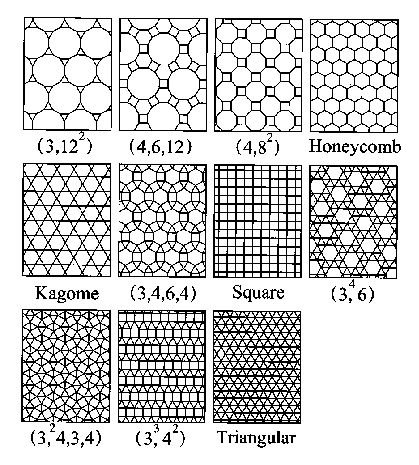
\includegraphics{./Einleitung-figs/archimed}
  \caption{Die elf archimedischen Gitter. Die Zahlenfolgen unter den Gitterausschnitten sind die Vertexkonfigurationen der Gitter, die keine gebr\"auchlichen Namen haben (siehe Text). Die Abbildung wurde aus \cite{Suding:99} \"ubernommen.}
  \label{fig:archimed}
\end{figure}
Da die Umgebungen aller Vertices bis auf eine Drehung identisch sind, lassen sich die Gitter durch die Folge $(n_1,\ldots,n_z)$ der Eckenzahlen der Polygone, die einen Vertex im Uhrzeigersinn umgeben, charakterisieren. Folgen $a_i$ gleiche Polygone aufeinander, so wird kurz $n_i^{a_i}$ geschrieben. Im Dreiecksgitter umgeben jeden Vertex sechs Dreiecke und die Vertexkonfiguration ist $(3^6)$. Analog sind die Vertexkonfigurationen des \mbox{Quadrat-,} des \mbox{Sechseck-} und des Kagom\'egitters,  $(4^4)$, $(6^3)$ bzw. $(3,6,3,6)$. F\"ur die \"ubrigen Gitter siehe Abb. \ref{fig:archimed}.
\\Die Euler-Charakteristik einer zweidimensionalen Figur ist die Differenz der Zahl der Komponenten der Figur und der Zahl der L"ocher in diesen Komponenten. Die mittlere Euler-Charakteristik $\chi(p)$ von Perkolationskonfigurationen auf Gittern ist also die mittlere Zahl der Cluster, abz\"uglich der mittleren Zahl der L\"ocher in diesen Clustern. Die mittlere Euler-Charakteristik des Quadratgitters ist links in Abbildung \ref{fig:chieinleit} dargestellt. Die mittleren Euler-Charakteristiken aller archimedischen Gitter sind bekannt \cite{Wagner:02}, und haben eine Nullstelle $p_0$ zwischen 0 und 1. Auch die site-Perkolationsschwellen $p_c$ aller archimedischen Gitter \cite{Suding:99} sind bekannt. Die Nullstelle $p_0$ liegt bei allen archimedischen Gittern knapp \"uber $p_c$. Dar\"uberhinaus liegt der Wendepunkt $p_0^{(2)}$ der Euler-Charakteristik knapp unter $p_c$, und das arithmetische Mittel aus Nullstelle und Wendepunkt liefert eine exzellente Approximation von $p_c$. Diese Befunde sind in  Tabelle \ref{tab:archisite} und Abbildung \ref{fig:archisite} zusammengetragen.\\
\begin{table}[htbp]
\centering
  \begin{tabular}{|l|r|r|r||r|}
    \hline
    Vertexkonfiguration &$p_0$ &$p_0^{(2)}$ &$\frac{p_0+p_0^{(2)}}{2}$& $p_c$ \cite{Suding:99} \\ \hline
    \hline

    $3,12^2$ &$0.8395$ &$0.7631$&$0.80131$&$0.8079$ \\ \hline

    $4,6,12$&$0.7833$ &$0.7012$ &$0.74227$&$0.7478$\\ \hline

    $4,8^2$&$0.7689$ &$0.6935$ &$0.73120$&$0.7292$\\ \hline

    $6^3$ Sechseckg. &$0.7413$&$0.6687$ &$0.70501$&$0.6970$\\ \hline

    $3,6,3,6$ Kagom\'eg.&$0.6756$&$0.6231$ &$0.64936$&$0.6527$ \\ \hline

    $3,4,6,4$ &$0.6468$&$0.5994$ &$0.62311$&$0.6218$ \\ \hline

    $4^4$ Quadratg.&$0.6180$&$0.5774$ &$0.59769$&$0.5927$\\ \hline

    $3^4,6$  &$0.5913$&$0.5625$  &$0.57686$& $0.5750$\\ \hline

    $3^2,4,3,4$ &$0.5616$ &$0.5408$ &$0.55119$&$0.5508$ \\ \hline

    $3^3,4^2$ &$0.5616$&$0.5408$ &$0.55119$&$0.5502$  \\ \hline

    $3^6$ Dreiecksg. &$\frac{1}{2}$&$\frac{1}{2}$&$\frac{1}{2}$ &$\frac{1}{2}$\\ \hline

    \hline
  \end{tabular}
  \caption{Euler-Charakteristik und site-Perkolation auf archimedischen Gittern: Die Nullstellen $p_0$ und die Wendepunkte $p_0^{(2)}$ der mittleren Euler-Charakteristik archimedischer Gitter sind obere bzw. untere Schranken f\"ur die site-Perkolationsschwellen $p_c$. Das arithmetische Mittel aus $p_0$ und $p_0^{(2)}$ ist eine exzellente Approximation von $p_c$.}
  \label{tab:archisite}
\end{table}
\begin{figure}[htbp]
  \centering
  \includegraphics[width=5.5in]{./Einleitung-figs/chi}
  \caption{Die mittlere Euler-Charakteristik pro Vertex $\chi(p)$ des zweidimensionalen Quadratgitters (links) und des dreidimensionalen einfach kubischen Gitters (rechts). Die Nullstelle $p_0$ von $\chi(p)$, die Perkolationsschwellen $p_c$ der Gitter, sowie im zweidimensionalen Fall der Wendepunkt $p_0^{(2)}$ von $\chi(p)$ sind jeweils markiert.}
  \label{fig:chieinleit}
\end{figure}


\begin{figure}[htbp]
  \centering
  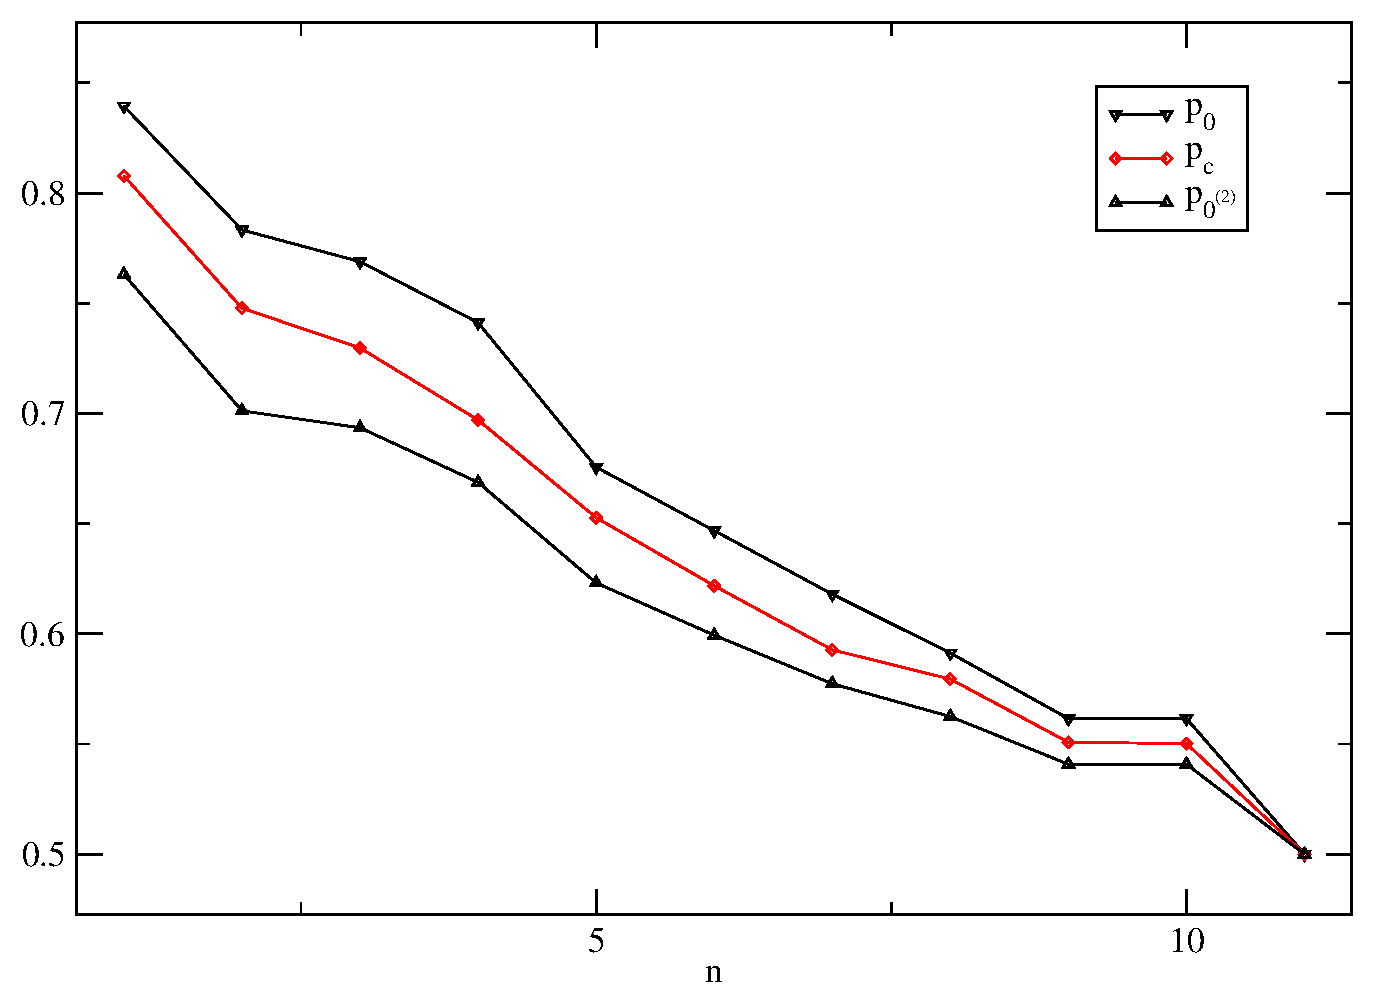
\includegraphics[width=5.5in]{./Einleitung-figs/archisitesingle}
  \caption{Die site-Perkolationsschwellen $p_c$ archimedischer Gitter liegen zwischen der Nullstelle $p_0$ und dem Wendepunkt $p_0^{(2)}$ der mittleren Euler-Charakteristik.}
  \label{fig:archisite}
\end{figure}


\subsection{Dreidimensionale Gitter}
Die Euler-Charakteristik einer dreidimensionalen Figur ist die Zahl der Komponenten, minus der Zahl der Henkel, plus der Zahl der Einschl"usse der Figur. F\"ur Perkolationskonfigurationen auf Gittern l\"asst sich eine mittlere Euler-Charakteristik $\chi(p)$ berechnen. In drei Dimensionen hat $\chi(p)$ zwei Nullstellen zwischen $0$ und $1$. Die mittlere Euler-Charakteristik ist f\"ur kleine $p$ (isolierte Cluster \"uberwiegen) und f\"ur $p$ nahe $1$ (Einschl\"usse \"uberwiegen) positiv. Zwischen diesen beiden Bereichen ist $\chi(p)$ negativ. Die mittlere Euler-Charakteristik des einfach kubischen Gitters ist rechts in Abbildung \ref{fig:chieinleit} dargestellt. Die kleinere Nullstelle der Euler-Charakteristik liegt beim einfach-kubischen (sc-) Gitter mit sechs und $26$ Nachbarn, beim fcc- mit $12$ und beim bcc-Gitter mit $14$ Nachbarn \"uber der Perkolationsschwelle (siehe Tabelle \ref{tab:3Dknown}). Der erste Wendepunkt von $\chi(p)$ liegt bei diesen Gittern \"uber der Perkolationsschwelle und liefert leider keine untere Schranke. 
\begin{table}[btp]
  \centering
  \begin{tabular}{|l|r|r||r|}
    \hline
    Gitter & \# Gitternachbarn &$p_0$ & $p_c$ \\ \hline
    sc & $6$  &$ 0.397 $& $0.3114(4)$ \\ \hline 
    sc & $26$ &$ 0.114 $& $0.097$  \\ \hline 
    bcc & $14$  &$ 0.211 $& $0.175$ \\ \hline 
    fcc & $12$  &$ 0.237 $& $0.1994(2)$ \\ \hline 

  \end{tabular}
  \caption{Dreidimensionale Gitter: Nullstellen $p_0$ der Euler-Charakteristik verglichen mit den Perkolationsschwellen $p_c$. Die Werte der Perkolationsschwellen des sc-Gitters mit 6 und des fcc-Gitter mit 12 Nachbarn stammen aus \cite{Marck:97}, die \"ubrigen aus \cite{Essam:72}. Letztere sind vermutlich sehr ungenau.}
  \label{tab:3Dknown}
\end{table}

\subsection{Hyperkubische Gitter}
Durch eine Rekursion l\"asst sich die mittlere Euler-Charakteristik hyperkubischer Gitter beliebiger Dimension $d$ ausrechnen (siehe Mecke \cite{Mecke:94} oder Jung \cite{Jung:00}). Aus
\begin{equation}
  \chi^d(p)=\sum_{i=0}^d (-1)^i{ d \choose i} p^{2^i}=p-dp^2+\frac{d(d-1)}{2}p^4-\cdots
\end{equation}
erh\"alt man f\"ur gro"se $d$ $p_0 \approx \frac{1}{d} =\frac{2}{z}$. Mit steigender Dimension des Gitters sollte sich die Perkolationsschwelle der des Bethe-Gitters $p_c=\frac{1}{z-1}$ ann\"ahern. Daher gilt f\"ur Perkolationsschwellen hoch-dimensionaler hyperkubischer Gitter $p_0\approx 2p_c$.


\subsection{Kontinuumsperkolation}
Mit Methoden der Integralgeometrie (\cite{Mecke:91} und \cite{Mecke:94}) kann die mittlere Euler-Charakteristik des Boolschen Kornmodells exakt bestimmt werden. Im Boolschen Kornmodell werden Punkte nach einem Poissonprozess mit Punktdichte $\rho$ verteilt und an diese Punkte unabh\"angig voneinander konvexe K\"orper angeheftet. Die mittlere Euler-Charakteristik h\"angt neben der Punktdichte $\rho$ auch von geometrischen Eigenschaften der K\"orper ab. In zwei Dimensionen geht das Verh\"altnis von Umfang $u$ und Fl\"ache $f$ der K\"orper in die Euler-Charakteristik ein, und mit $I=\frac{u^2}{4\pi f}$ erh\"alt man f\"ur die Euler-Charakteristik pro Fl\"ache
\begin{equation}
  \chi_2(\eta)=\eta(1 - I\eta)e^{-\eta}.
\end{equation}
Hier ist $\eta$ das Produkt aus $\rho$ und der Fl\"ache der K\"orper. In drei Dimensionen h\"angt $\chi$ vom Verh\"altnis der Oberfl\"ache $f$ und der mittleren integralen Kr\"ummung $h$ zum Volumen $v$ ab. Mit $I_1=\frac{fh}{12\pi v}$, $I_2=\frac{f^3}{36\pi v^2}$ und $\eta=\rho v$ ist die Euler-Charakteristik pro Volumen 
 \begin{equation}
  \chi_3(\eta)=\eta(1-3I_1\eta + \frac{3\pi^2}{32}I_2\eta^2)e^{-\eta}.
\end{equation}
 \\
Die Perkolationsschwellen $\eta_c$ des Boolschen Kornmodells monodisperser Kugeln ist in zwei und drei Dimensionen numerisch bekannt und die Nullstelle $\eta_0$ von $\chi_d(\eta)$ liegt zwei Dimensionen knapp unter und in drei Dimensionen knapp \"uber $\eta_c$.\\

\noindent
Auf Kontinuumsperkolation und hyperkubische Gitter wird im Folgenden nicht mehr eingegangen. Sie werden hier nur der Vollst\"andigkeit halber beschrieben. In dieser Arbeit werden die empirischen Beobachtungen, dass
\textbf{ %
\begin{itemize}
\item die Perkolationsschwellen zweidimensionaler Gitter zwischen der Nullstelle und dem Wendepunkt der mittleren Euler-Charakteristik liegen,
\item  die Nullstelle der mittleren Euler-Charakteristik dreidimensionaler Gitter \"uber deren Perkolationsschwelle liegt,
\end{itemize} %
}
\noindent untersucht. Im folgenden Kapitel wird zun\"achst die Euler-Charakteristik genauer betrachtet.
